% =====================================================================
% Figure: Method positioning matrix — AEGIS vs prior structural-vulnerability
% analyses. Closes editorial decision item C-DA2 (defuses the "strawman gap").
%
% Citation numbers are local to this figure:
%   [1] Nettack: Zuegner et al. 2018  \cite{zugner2018adversarial}
%   [2] Mettack: Zuegner et al. 2019  \cite{zugner2019adversarial}
%   [3] GR-BCD:  Geisler et al. 2021  \cite{geisler2021robustness}
%   [4] Localized smoothing: Schuchardt et al. 2023 \cite{schuchardt2023localized}
%   [5] AGNNCert: Li et al. 2025      \cite{li2025agnncert}
% Add this mapping to the caption when including the figure.
%
% Design notes (revision pass):
%   - Increased row spacing so method labels don't crowd each other.
%   - Reserved a 2-line header zone with explicit \\ line breaks so the
%     longest header ("Realistic / Edge-only perturbation") fits cleanly.
%   - Pushed the header rule far enough below the headers and far enough
%     above the first row that no label overlaps with the rule.
%   - Added zebra row shading for visual separation between rows.
%   - Kept the AEGIS row's full-width green band for the "we cover all
%     four columns" punchline.
% =====================================================================

\documentclass[tikz,border=3pt,11pt]{standalone}
\usepackage[T1]{fontenc}
\usepackage{mathptmx}
\usepackage{tikz}
\usetikzlibrary{shapes.geometric, positioning, calc, fit, backgrounds}
\usepackage{xcolor}
\usepackage{amsmath, amssymb}
\usepackage{xspace}
\newcommand{\AEGIS}{\textsc{Aegis}\xspace}
\renewcommand{\familydefault}{\rmdefault}

\definecolor{cattack}{HTML}{D55E00}    % vermilion -- attack methods
\definecolor{ccert}{HTML}{0072B2}       % blue      -- certifiers
\definecolor{caegis}{HTML}{009E73}      % green     -- AEGIS
\definecolor{caegisbg}{HTML}{D5F0E2}    % light tint of caegis for band
\definecolor{czebra}{HTML}{F4F4F4}      % zebra-stripe background
\definecolor{ckey}{HTML}{6E6E6E}        % grey for citation numbers

% --- A "supported" pill: filled coloured dot + short label
\newcommand{\support}[2]{%
  \tikz[baseline=-0.6ex]{\fill[#1] (0,0) circle (1.8pt);}\,%
  \textcolor{#1}{\normalsize #2}%
}
% --- Citation tag in grey
\newcommand{\citetag}[1]{{\color{ckey}\normalsize[#1]}}

\begin{document}
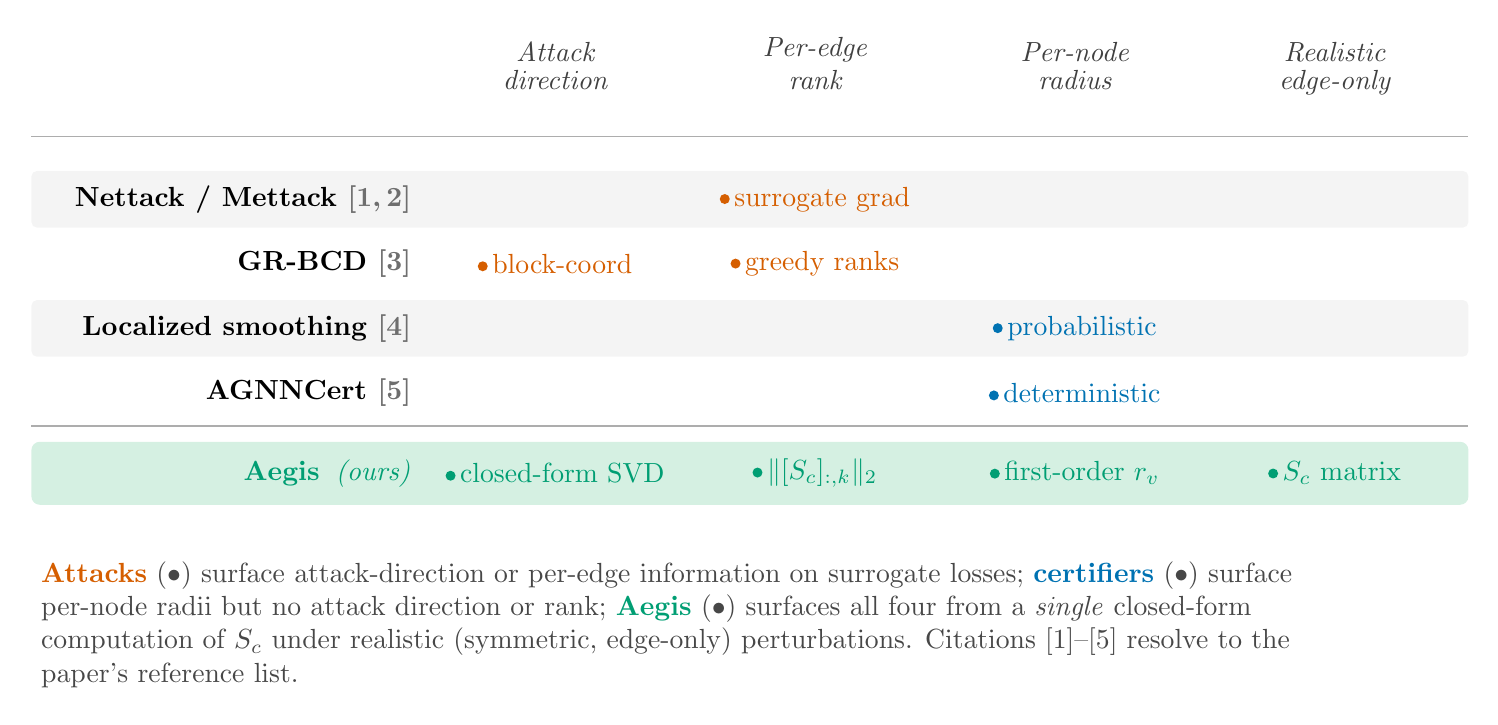
\begin{tikzpicture}[
    font=\rmfamily,
    %% Layout constants -------------------------------------------------
    %% Wider cell + method columns so single-line strings ("closed-form SVD",
    %% "Nettack / Mettack [1, 2]", "Localized smoothing [4]") do not wrap
    %% or hyphenate. Hyphenation is also suppressed inside cell text.
    cw/.style={text width=3.20cm, align=center},
    head/.style={cw, align=center, font=\rmfamily\normalsize\itshape,
                  text=black!75, anchor=center},
    method/.style={anchor=east, align=right, font=\rmfamily\normalsize\bfseries,
                   text width=4.80cm, inner sep=2pt},
    cell/.style={cw, align=center, font=\rmfamily\normalsize,
                  anchor=center, inner sep=2pt},
]
% Suppress automatic hyphenation everywhere in this figure -- prevents
% awkward breaks like "Met-tack" and "closed- form SVD".
\hyphenpenalty=10000\relax
\exhyphenpenalty=10000\relax

%% ----- coordinates ---------------------------------------------------
\def\rowH{0.82}    % row spacing -- bumped from 0.62 to 0.82 for breathing room
\def\colA{0.0}
\def\colB{3.30}
\def\colC{6.60}
\def\colD{9.90}
\pgfmathsetmacro{\xLab}{-1.75}
\pgfmathsetmacro{\xLeft}{-6.65}
\pgfmathsetmacro{\xRight}{11.60}

%% Header zone: reserve TWO lines + padding above the rule so the longest
%% header ("Realistic / Edge-only perturbation") never collides with the
%% rule or the first method row.
\pgfmathsetmacro{\yHeadTop}{0.55}    % top of header (line 1)
\pgfmathsetmacro{\yHeadBot}{0.05}    % bottom of header (line 2)
\pgfmathsetmacro{\yRule}{-0.55}      % separator rule beneath the header zone
\pgfmathsetmacro{\yA}{-1.35}         % first method row -- well clear of the rule
\pgfmathsetmacro{\yB}{\yA - \rowH}
\pgfmathsetmacro{\yC}{\yB - \rowH}
\pgfmathsetmacro{\yD}{\yC - \rowH}
\pgfmathsetmacro{\yE}{\yD - \rowH - 0.20}   % extra gap before AEGIS

%% ----- zebra row shading (drawn on background) ----------------------
\begin{scope}[on background layer]
  \fill[czebra, rounded corners=2pt]
    (\xLeft, \yA + 0.36) rectangle (\xRight, \yA - 0.36);
  \fill[czebra, rounded corners=2pt]
    (\xLeft, \yC + 0.36) rectangle (\xRight, \yC - 0.36);
\end{scope}

%% ----- header row (each header anchored at its bottom-of-line-2) -----
%% Use explicit two-line headers via \shortstack so column 4 stays inside
%% its 2.85cm slot without an ad-hoc wrap.
\node[head, anchor=base] at (\colA, \yHeadBot)
    {\shortstack{Attack\\direction}};
\node[head, anchor=base] at (\colB, \yHeadBot)
    {\shortstack{Per-edge\\rank}};
\node[head, anchor=base] at (\colC, \yHeadBot)
    {\shortstack{Per-node\\radius}};
\node[head, anchor=base] at (\colD, \yHeadBot)
    {\shortstack{Realistic\\edge-only}};

%% ----- AEGIS row background band -- covers the FULL row, label too --
\begin{scope}[on background layer]
  \fill[caegisbg, rounded corners=3pt]
    (\xLeft, \yE - 0.40) rectangle (\xRight, \yE + 0.40);
\end{scope}

%% ----- row labels (single line, [N] citation inline) ----------------
\node[method] at (\xLab, \yA) {Nettack / Mettack~\citetag{1,\,2}};
\node[method] at (\xLab, \yB) {GR-BCD~\citetag{3}};
\node[method] at (\xLab, \yC) {Localized smoothing~\citetag{4}};
\node[method] at (\xLab, \yD) {AGNNCert~\citetag{5}};
\node[method, text=caegis] at (\xLab, \yE)
    {\AEGIS\,\textnormal{\itshape\normalsize(ours)}};

%% ----- prior-method cells -------------------------------------------
% Row 1: Nettack/Mettack -- only per-edge rank
\node[cell] at (\colB, \yA) {\support{cattack}{surrogate grad}};

% Row 2: GR-BCD -- attack direction + per-edge rank
\node[cell] at (\colA, \yB) {\support{cattack}{block-coord}};
\node[cell] at (\colB, \yB) {\support{cattack}{greedy ranks}};

% Row 3: Localized smoothing -- per-node radius (probabilistic)
\node[cell] at (\colC, \yC) {\support{ccert}{probabilistic}};

% Row 4: AGNNCert -- per-node radius (deterministic)
\node[cell] at (\colC, \yD) {\support{ccert}{deterministic}};

%% ----- AEGIS row cells (all four supported) -------------------------
\node[cell] at (\colA, \yE) {\support{caegis}{closed-form SVD}};
\node[cell] at (\colB, \yE) {\support{caegis}{$\|[S_c]_{:,k}\|_2$}};
\node[cell] at (\colC, \yE) {\support{caegis}{first-order $r_v$}};
\node[cell] at (\colD, \yE) {\support{caegis}{$S_c$ matrix}};

%% ----- horizontal rules ----------------------------------------------
% Under header (well below the header text, well above first row)
\draw[black!32, line width=0.5pt] (\xLeft, \yRule) -- (\xRight, \yRule);
% Above AEGIS band
\draw[black!32, line width=0.5pt]
    (\xLeft, \yD - 0.42) -- (\xRight, \yD - 0.42);

%% ----- legend caption (in grey, below) ------------------------------
\node[anchor=north west, font=\rmfamily\normalsize, text=black!72]
     at (\xLeft, \yE - 1.00) {%
   \begin{minipage}{16.2cm}\raggedright
   \textcolor{cattack}{\textbf{Attacks}} ($\bullet$) surface attack-direction
   or per-edge information on surrogate losses;
   \textcolor{ccert}{\textbf{certifiers}} ($\bullet$) surface per-node radii
   but no attack direction or rank;
   \textcolor{caegis}{\textbf{\AEGIS}} ($\bullet$) surfaces all four
   from a \emph{single} closed-form computation of $S_c$ under realistic
   (symmetric, edge-only) perturbations. Citations~[1]--[5] resolve to
   the paper's reference list.
   \end{minipage}};

\end{tikzpicture}
\end{document}
